\section{Micro-Frontend Architecture}\label{section:background:micro-frontend-architecture}

Micro-frontends should bring the same advantages of microservices to the frontend. Instead of creating a giant frontend monolith, a micro-frontend architecture contains many small applications. The advantage is that a separate team can develop and deploy every micro-frontend independently. \cite{book:2020:geers:background:micro-frontends:micro-frontends-in-action} The difference between monolithic frontend architecture and micro-frontend architecture can be seen in the Figure \ref{fig:background:micro-frontend:monolith-micro-frontend-comparison}.

\ifshowImages
\begin{figure}[H]
    \centering
    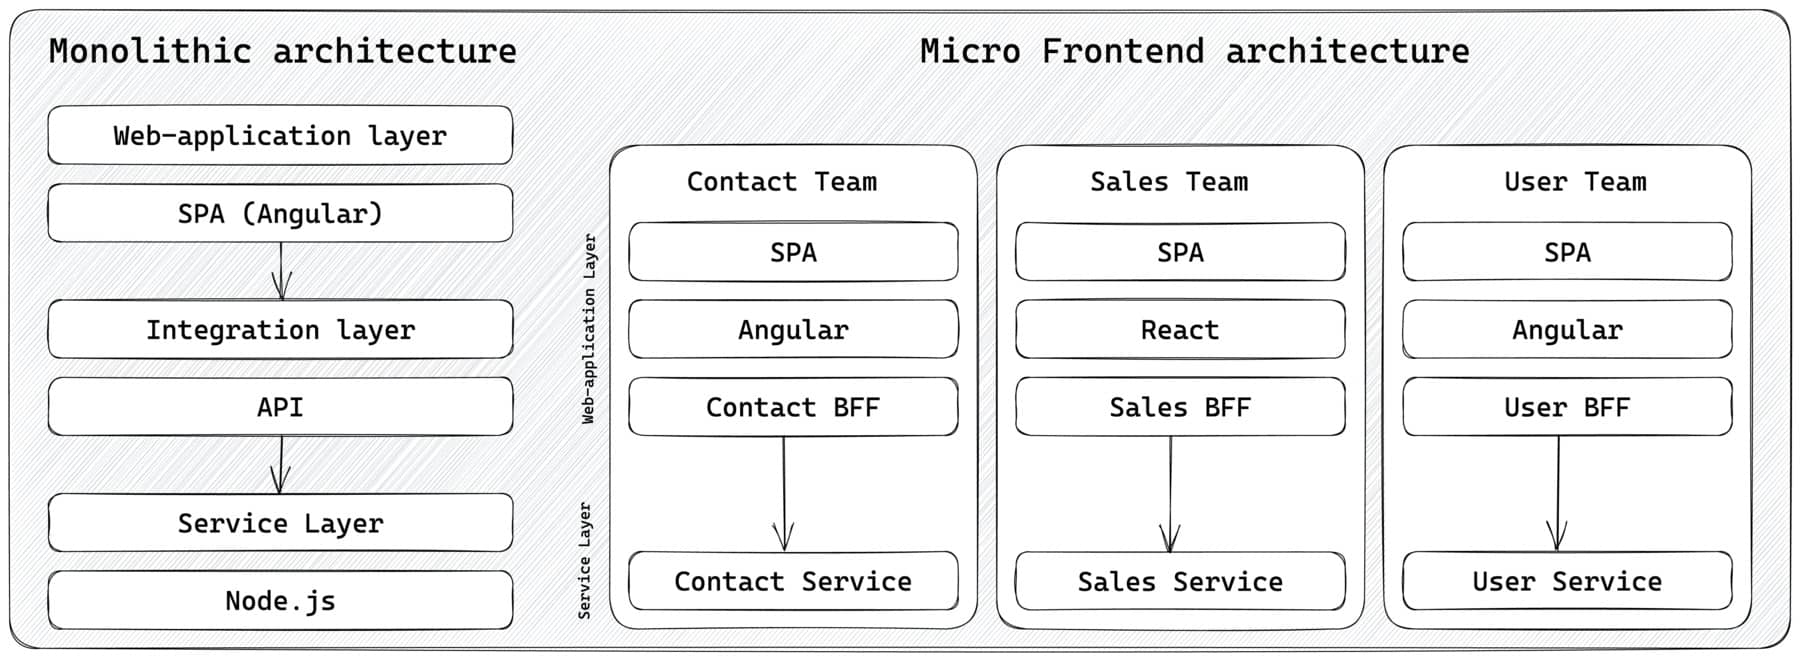
\includegraphics[width=1\linewidth]{images/background/micro-frontends/monolith-micro-frontends-comparison.jpg}
    \caption{A comparison between frontend-monoliths and micro-frontends.}\label{fig:background:micro-frontend:monolith-micro-frontend-comparison}
\end{figure}
\fi

\noindent Benefits gained from working with microservices are lost when working with a monolithic frontend. With a monolithic frontend, the ability to deploy independently is lost. The entire frontend has to be deployed at once. Another problem is that distinct operations are not possible. If one part of the frontend is broken, there is a good chance that the entire frontend does not work. Another problem is parallel development. The development speed cannot be increased because having multiple teams working on one frontend application is very difficult. \cite{misc:2019:leitner:background:micro-frontends:micro-frontends-basics}

\bigskip

\noindent The term micro-frontend can be misleading, as can the term microservice. It has no meaning in terms of the size of the application, and it can be a simple widget that only displays data or a full-blown single-page application. Ideally, a micro frontend covers an area of the entire frontend application.

\bigskip

\noindent Micro-frontends apply the same principles from the microservice architecture to frontend development. Often a microservice architecture developed by several teams has only one frontend monolith. Therefore, when adding new features, a single team can be overwhelmed. Like a microservice architecture, a micro-frontend architecture focuses on developing many small frontend applications instead of developing a giant software monolith. Each micro-frontend can be developed independently by another team. However, a challenge is that the micro-frontend should appear as a single application to the user. Therefore, the different applications must be integrated, which can be challenging.

\bigskip

\noindent Building micro-frontends with the web allows different strategies for integrating the applications. Three strategies exist to combine multiple micro-frontends into an application shell: client-side integration, server-side integration, and the combination of these two strategies. \cite[10-12]{book:2020:geers:background:micro-frontends:micro-frontends-in-action}

\subsection{Characteristics}\label{subsection:background:micro-frontend-characteristics}

Micro-frontends follow the same characteristics as microservices, described in more detail in this chapter.

\subsubsection{Autonomous}\label{subsubsection:background:micro-frontend-autonomous}

Technically a micro-frontend is an entirely independent and runnable application. The integration of the micro-frontends happens only through the frontend. The different micro-frontends are composed within an application shell. The application shell is a separate application that is usually the entry point for the user to interact with all micro-frontends. The application shell also provides the page layout and defines where the micro-frontends are displayed. Autonomy should not go in the direction of complete isolation. Nevertheless, no dependencies should emerge, which could harm autonomy. \cite{book:2020:geers:background:micro-frontends:micro-frontends-in-action}

\subsubsection{Technology Agnostic}\label{subsubsection:background:micro-frontend-technology-agnostic}

Just as microservice architectures, micro-frontend architectures can be technology agnostic. The current frontend development landscape offers a lot of \ac{JS} frameworks, which offer different advantages and disadvantages. The advantage of an application with small independent building blocks is that parts can be rewritten with another technology more efficiently. \cite[14-16]{book:2020:geers:background:micro-frontends:micro-frontends-in-action} However, using different technologies for different micro-frontends can lead to problems with the chosen form of integration and communication. The communication should also be technology agnostic and use browser-native tools like Broadcast Channel \ac{API}.

\bigskip

\noindent Another problem that could arise is the bundle size of modern \ac{JS} frameworks. If two frameworks like React and Angular need to be fetched, the total bundle size can be enormous and a strain on (mobile) network connections. Loading and running multiple micro-frontends is also resource intensive. Micro-frontends can be developed using a standardized \ac{API} like Web Components. With this approach, no specific framework is needed for developing the application. \cite{book:2020:geers:background:micro-frontends:micro-frontends-in-action}

\subsubsection{Independently Deployable}\label{subsubsection:background:micro-frontend-independent-deployable}

The autonomy of micro-frontends offers the possibility for independent deployments. A sizeable monolithic frontend application is more complex to deploy, and there is no need for communication and coordination over multiple teams to deploy the application. Organizational dependencies negatively impact the time-to-market because development teams would have to wait for another team's release. \cite[12]{book:2020:geers:background:micro-frontends:micro-frontends-in-action}

\subsubsection{Small and Easy to Maintain}\label{subsubsection:background:micro-frontend-small-and-easy-to-maintain}

Because micro-frontends only cover a small domain of an application, the source code is smaller and easier to understand. A smaller codebase is especially helpful for understanding the inner workings of the software. Onboarding new team members is also more accessible because the codebase is smaller than monoliths.
Due to the easier understanding of the domain, the application can be easier rewritten with state-of-the-art technology if the old one becomes deprecated. \cite{book:2020:geers:background:micro-frontends:micro-frontends-in-action}

\subsubsection{Resilience}\label{subsubsection:background:micro-frontend-resilience}

Micro-frontends offer the possibility of building an application by composing multiple independent small applications into fully-fledged ones. Depending on the integration strategy, micro-frontends are usually combined at runtime. However, the network, especially for mobile devices, sometimes fails. A micro-frontend architecture provides better failure isolation. One micro-frontend crashing does not affect the other micro-frontends inside the application. Some parts of the application might not work, but other parts of the application are still usable. The application shell can react to a failure and tell users that the application is not working as expected and will be available soon. \cite[10-11]{article:2021:perltonen:background:micro-frontends:motivations-benefits-and-issues}

\subsection{Disadvantages}\label{subsection:background:micro-frontend-downsides}

Building micro-frontends comes with many advantages but also with some downsides. The following section describes some disadvantages of micro-frontends. The autonomy of having independent teams that build autonomous software comes with a price. A critical aspect of building software is eliminating redundancy in the code, and having multiple teams that build and run applications might introduce much redundancy. Moreover, if the \ac{BFF} pattern is used, the services to deploy increase even more, significantly increasing infrastructure complexity. Every team must set up its build process and a continuous integration pipeline. Duplicate \ac{CSS} and \ac{JS} code might be shipped to the browser. If multiple teams use a popular library and a critical security vulnerability is encountered, every team must update the dependency and deploy the application to fix the problem. It is essential to share knowledge between the teams to avoid fixing the same bugs repeatedly. The cost of having redundancies is lower than the negative impacts of having inter-team dependencies. The free choice of technology also comes with some disadvantages. It is hard for a developer to switch from one team to another or exchange their best practices for development. Like in distributed systems, keeping backward compatibility between the different micro-frontends takes much work. Different micro-frontends have different dependencies, versions, and interfaces.  \cite[17-18]{book:2020:geers:background:micro-frontends:micro-frontends-in-action} One of the main concerns is payload size, as independently-built JavaScript bundles can cause duplication of common dependencies, increasing the number of bytes sent over the network to end users. Additionally, maintaining consistency in user experience and visual design across different micro-frontends can take time, especially when developed by different teams or technologies. Maintaining a consistent look and feel across different components, like a Design System, can require additional effort and coordination. \cite{misc:2019:jackson:background:micro-frontends:disadvantages} Another problem addressed in this master thesis is the problem of over-fetching and over-requesting. Multiple micro-frontends might make exactly the same requests to the \ac{BFF}, leading to a higher server load. If a traditional \ac{REST} service is used, a micro-frontend might need to make more requests to fetch the desired data, while another might need precisely that data. 

% Another difficulty is how to slice micro-frontends. The micro-frontends should not depend on each other during runtime.

\subsection{Integration strategies}\label{subsection:background:micro-frontend-architecture:integration-strategies}

Micro-frontends can be integrated with different strategies. The integration strategy depends on the requirements of the system. They can be composed using a client-side integration strategy, a server-side strategy, or a combination of both.

\subsubsection{Server-Side Integration}\label{subsubsection:background:micro-frontend-architecture:integration-strategies:server-side-integration}

A Service between the client and the backend usually does server-side composition. \cite[60]{book:2020:geers:background:micro-frontends:micro-frontends-in-action} The server responds with references to micro-frontends that should be included and their required assets. The service in the middle intercepts that response and replaces the references to the micro-frontends with the actual content before the response is sent to the browser. The micro-frontends are included in their position and later appear in the HTML. An example of a server-side include can be seen in listing \ref{code:background:micro-frontends:server-side-include}. The other micro-frontends are referenced with URLs. \cite[61-63]{book:2020:geers:background:micro-frontends:micro-frontends-in-action}

\ifshowListings
\begin{listing}[H]
    \begin{minted}{html}
<html>
  <body>
    <!--#include virtual="/erp/dashboard" -->
  </body>
</html>
    \end{minted}
    \caption{An example server-side include.}\label{code:background:micro-frontends:server-side-include}
\end{listing}
\fi

\bigskip

\noindent One advantage of server-side integration is the fast first-load performance, which is the principle of progressive enhancement. \cite{book:2010:parker:background:micro-frontends:designing-with-progressive-enhancement} The browser fetches the HTML and renders it. It does not have to assemble parts of a page, like with client-side integration. The computation is only done on the server, which reduces the strain on the user's device. \cite{book:2020:geers:background:micro-frontends:micro-frontends-in-action} However, assets like stylesheets and images must still be fetched from the server. Server Side Integration is helpful if the application's primary concern is presenting static content to the end user and instant reaction to the users' inputs is unnecessary.  \cite[83]{book:2020:geers:background:micro-frontends:micro-frontends-in-action}

\subsubsection{Client-Side Integration}\label{subsubsection:background:micro-frontend-architecture:integration-strategies:client-side-integration}

When the application should react promptly to user input, a client-side integration strategy is preferred. For example, when developing an online marketplace, the user should be able to add items to the cart without making a complete roundtrip to the server to see the updated value. The application should provide a seamless user experience, as the end user just uses one application. Modern Frameworks like Angular and React offer the development of Single Page Applications, which provide reactive, client-side rendered applications. The HTML Markup is produced on the client instead of the server. \cite{book:2020:geers:background:micro-frontends:micro-frontends-in-action}

\bigskip

\noindent Client-side integration can be achieved through different approaches. The most straightforward approach combines the micro-frontends by linking the different applications with Hyperlinks. Each micro-frontend is deployed and accessible via a different URL, and the different micro-frontend applications are then linked with Hyperlinks. As the approach implies, switching to another micro-frontend requires a complete page reload and a roundtrip to the server. However, the integration with Hyperlinks breaks the SPA approach. This strategy makes it necessary that every micro-frontend is accessible via its URL and that it can be served as a standalone application.

\bigskip

\noindent Another client-side approach is to combine micro-frontend with iFrames or Web-Components. Integrating micro-frontends with this approach enables the page to be a SPA still. The client can navigate multiple micro-frontends without noticing, and no page reloads are needed. An iFrame is an isolated area with its own browser context \cite[35]{book:2020:geers:background:micro-frontends:micro-frontends-in-action}, Web Components are self-created HTML elements that are embedded into the DOM of the browser \cite[103]{book:2019:farrell:background:micro-frontends:web-components-in-action}. Integrating applications with the client-side strategy using Module Federation is explained in more detail in section \ref{subsubsection:background:micro-frontend:module-federation:101}.


\subsection{Communication between Micro-frontends}

Micro-frontends should not depend on each other. But it is necessary to have communication between them. For example if a user adds an item to a shopping-cart in an e-commerce application, the product micro-frontend has to inform the shopping-cart micro-frontend, which item was added. To reduce the coupling between applications and development teams it is recommended to keep the communication between micro-frontends at a minimum. Before choosing a communication pattern it is important to know the type of communication. If communication between two micro-frontends or between the app shell and a micro-frontend is required, the communication can take place via the user interface. Other communication mechanisms, like the Broadcast Channel API provided by the browser, are useful for state sharing or for passing on information to multiple micro-frontends. \cite{book:2020:geers:background:micro-frontends:micro-frontends-in-action}

\bigskip

\noindent When the micro-frontends are integrated via hyperlinks, the communication can only happen via URL parameters. Single-Page-Applications usually communicate via custom events and attribute changes of the components. \cite[100]{book:2020:geers:background:micro-frontends:micro-frontends-in-action} \cite[315-316]{book:2019:farrell:background:micro-frontends:web-components-in-action} A distinction can be made between \textbf{parent-to-fragment}, \textbf{fragment-to-parent} or \textbf{fragment-to-fragment} communication, where the term fragment is equivalent to a micro-frontend and the term parent is equivalent to the app shell. \cite{book:2020:geers:background:micro-frontends:micro-frontends-in-action} This is further shown in figure \ref{fig:background:micro-frontend:communication:communication-patterns}

\ifshowImages
\begin{figure}[H]
    \centering
    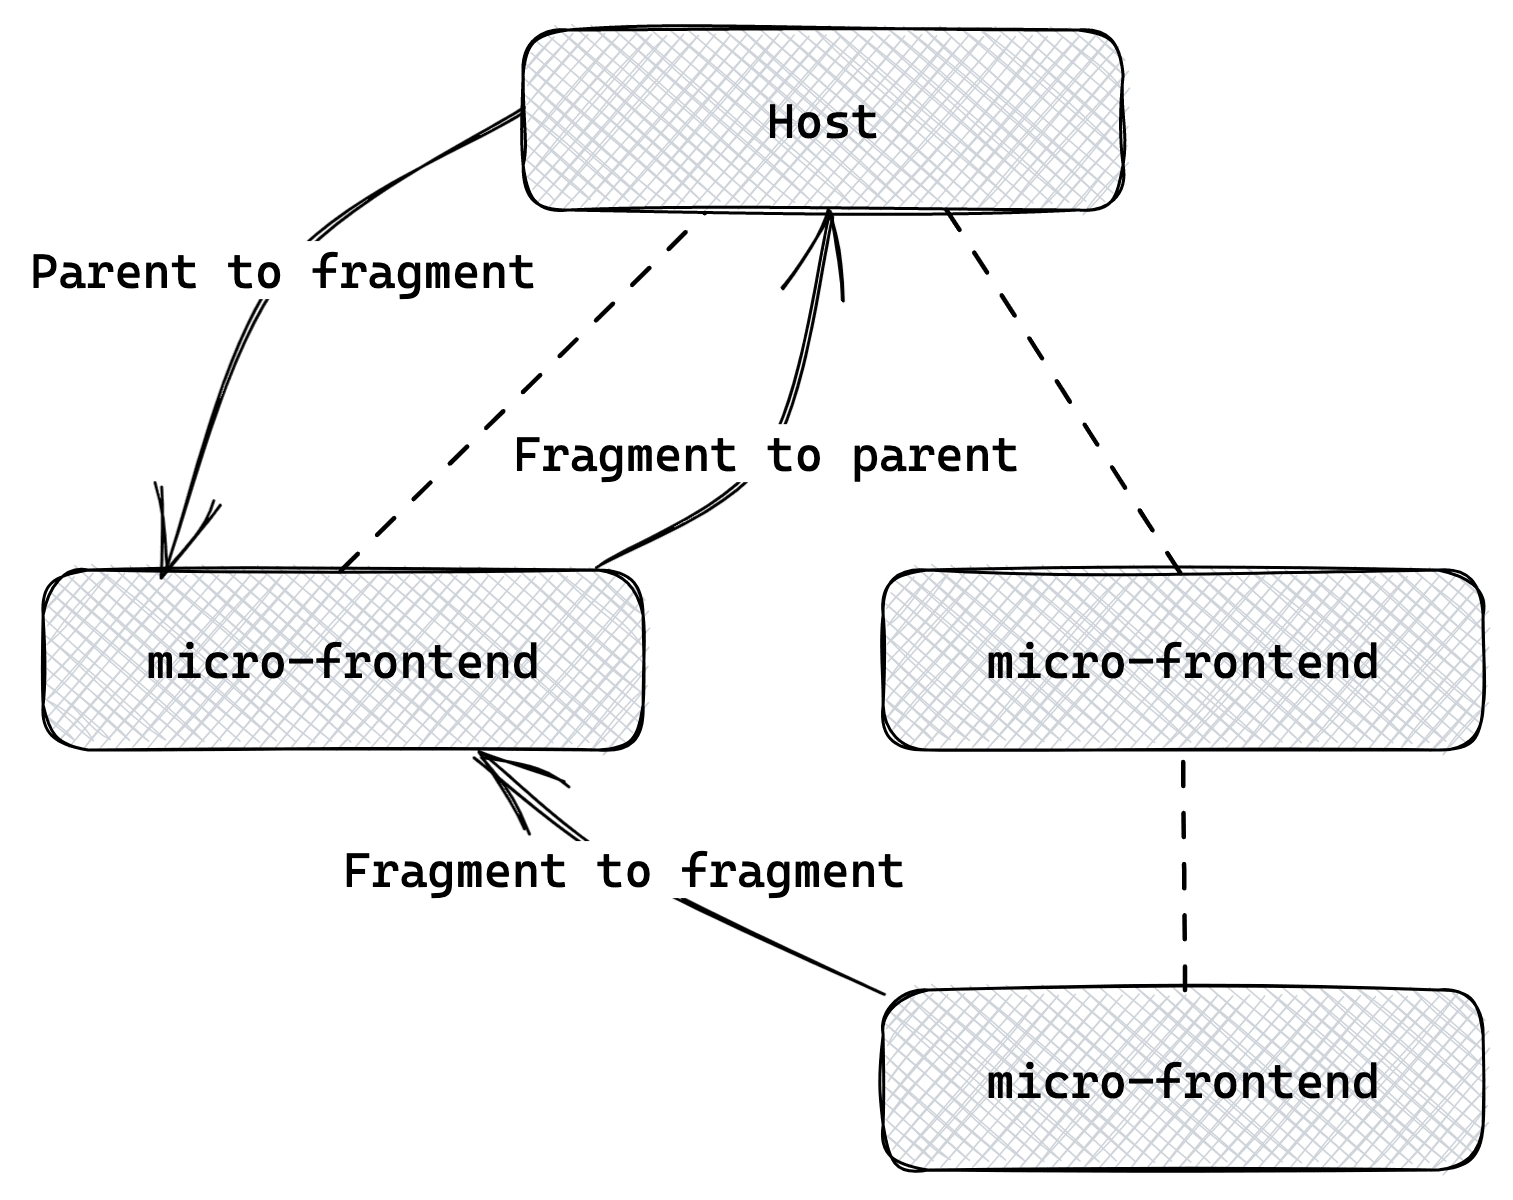
\includegraphics[width=0.5\linewidth]{images/background/communication/communication-patterns.png}
    \caption{Different forms of communication in micro-frontend architectures (Adapted from \cite[100]{book:2020:geers:background:micro-frontends:micro-frontends-in-action})}\label{fig:background:micro-frontend:communication:communication-patterns}
\end{figure}
\fi

\bigskip

\noindent Parent-to-fragment communication can happen via attribute changes when using Web Components. \cite[58-59]{book:2019:farrell:background:micro-frontends:web-components-in-action} To pass data from a micro-frontend to the app shell, custom-events can be used. \cite[315]{book:2019:farrell:background:micro-frontends:web-components-in-action}, where the micro-frontend emits an event, that the app shell is subscribed to. \cite{book:2020:geers:background:micro-frontends:micro-frontends-in-action}

\bigskip

\noindent Fragment-to-fragment communication is required when two micro-frontends should communicate with each other. The changes of one micro-frontend should have an effect on the other micro-frontend. This form of communication can be implemented in three ways: \cite[107-108]{book:2020:geers:background:micro-frontends:micro-frontends-in-action}

\begin{itemize}
    \item \textbf{Direct communication}: This is the most direct form of communication. One micro-frontend changes the attributes of its HTML elements with JavaScript. This approach is not recommended, because it introduces high coupling between two micro-frontends. One micro-frontends needs to know implementation details of the other micro-frontend. This makes it difficult to change the implementation of one micro-frontend without breaking the other micro-frontend. And this breaks one characteristics of micro-frontends, which are independent and autonomous development and deployment.
    \item \textbf{Orchestration via a parent}: When using this approach, the app shell is responsible for the communication between micro-frontends. One micro-frontend emits an event, which is intercepted by the app-shell. The app-shell sends the event to the target micro-frontend. This approach allows the micro-frontends to be completely decoupled, but changes have to be adapted by every micro-frontend.
    \item \textbf{Event-Bus/broadcasting}: Instead of a direct communication between micro-frontends or an indirect communication via the app-shell, a micro-frontend can publish an event on a central event-bus. The other micro-frontends can subscribe to the event and react to it. This is described as publish/subscribe mechanism. This drastically reduces the coupling between micro-frontends. No micro-frontend needs any information about the other micro-frontends, which allows perfect parallel development.
\end{itemize}


\subsection{Module Federation}\label{subsection:background:micro-frontend:module-federation}

Webpack 5 introduced a new native plugin called Module Federation. Module Federation allows chunks of \ac{JS} code to be loaded synchronously or asynchronously during runtime, allowing multiple teams to work in isolation and take care of the application composition. Lazy-loading different \ac{JS} chunks take place behind the scenes. \cite[81]{book:2021:mezzalira:applied-methods:building-micro-frontends}

\bigskip

\noindent Typically a module-federation application consists of two parts: \cite[81]{book:2021:mezzalira:applied-methods:building-micro-frontends}

\begin{itemize}
  \item The \texttt{host}, which is the main application is therefore responsible for loading the remote micro-frontends or libraries.
  \item The \texttt{remote}, which is either a micro-frontend or library, is consumed by the host. A remote can expose multiple modules that can be lazy-loaded inside the application.
\end{itemize}

\noindent Exposing micro-frontends or libraries with Module Federation is very simple, and developers can import the remote micro-frontends and compose the view as they would with normal modules. Another essential feature of Module Federation for micro-frontend architectures is the possibility of sharing the same instance of external dependencies across all micro-frontends. If a library should be shared across multiple micro-frontends, Module Federation will make sure to load only one instance. For example, if all micro-frontends should use version 15 of Angular, the version of the shared dependency has to be specified in the Module Federation configuration. At run time, Webpack will load only one version of Angular for all micro-frontends that use it. Working with different versions of the same library is also possible, and Module Federation will put each version in a different scope to avoid clashes at runtime. Module Federation is not just limited to the client but is also viable if the application is rendered on the server. \cite[82-83]{book:2021:mezzalira:applied-methods:building-micro-frontends}

\subsubsection{Performance}\label{subsubsection:background:micro-frontend:module-federation:performance}

Image multiple teams working on the same application. Each team develops one or more micro-frontend, and the teams have agreed to use the same \ac{UI} component libraries for the micro-frontend architecture. These libraries can be automatically shared with Module Federation, and they will be loaded only once at the beginning of the project, therefore all projects have the same version of the \ac{UI} components. Using only one instance of a dependency for multiple applications saves the browser from downloading a large \ac{JS} bundle. Module Federation can also load new micro-frontends during runtime, instead of defining them all in the configuration. \cite[83]{book:2021:mezzalira:applied-methods:building-micro-frontends}

\subsubsection{Composition}\label{subsubsection:background:micro-frontend:module-federation:composition}

Using Module Federation is as easy as importing external \ac{JS} chunks lazy-loaded inside a project. Lazy loading describes a technique, that defers the loading of resources until they are needed. The technique is especially important in web development to reduce the time until a page is rendered initially. Resources like images are loaded only when they are visible on the screen. The composition of applications occurs on the client side at runtime, when an application shell is used for loading different micro-frontends, or on the server when a server-side rendered application is used. \cite[84]{book:2021:mezzalira:applied-methods:building-micro-frontends}

\subsubsection{Shared code}\label{subsubsection:background:micro-frontend:module-federation:shared-code}

Module Federation makes sharing code between multiple teams very easy. Module federation allows sharing code between multiple micro-frontends bidirectional. This Webpack plugin flattens the hierarchy between the application shell and the remote micro-frontends. But sharing code from micro-frontends to the host application is discouraged because a unidirectional implementation brings several advantages such as the following: \cite[84]{book:2021:mezzalira:applied-methods:building-micro-frontends}

\begin{itemize}
  \item The code is easier to debug, as the location of the code is known.
  \item It is less prone to errors, and the code communicates in controllable ways.
  \item It is more efficient, as the micro-frontend knows the boundaries of each part of the application.
\end{itemize}

\subsubsection{Module Federation 101}\label{subsubsection:background:micro-frontend:module-federation:101}

Module Federation allows a \ac{JS} application to dynamically load and run code from another bundle. Module Federation provides two key concepts that are very important before working with it. \cite[118-119]{book:2021:mezzalira:applied-methods:building-micro-frontends}

\begin{itemize}
    \item \texttt{Host}: The host is the that container loads the shared libraries and micro-frontends at runtime.
    \item \texttt{Remote}: The bundle that should be consumed by the host.
\end{itemize}

\noindent Figure \ref{fig:background:micro-frontend:module-federation:module-federation-architecture} shows a host application that loads multiple remotes. The host is also called an application shell, whereas a remote is a micro-frontend.

\ifshowImages
\begin{figure}[H]
  \centering
  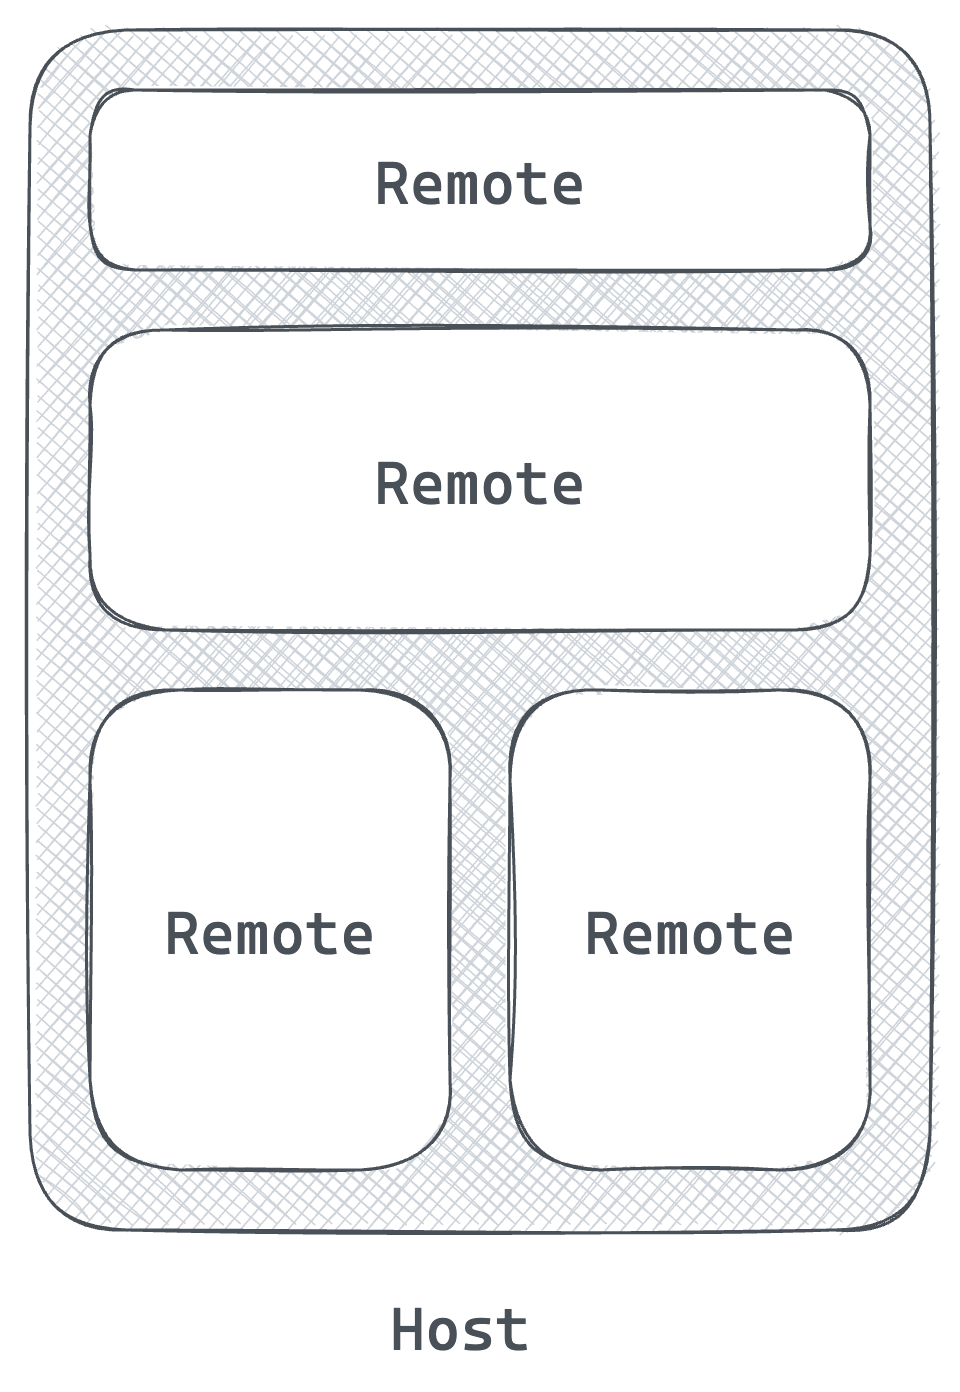
\includegraphics[width=0.3\linewidth]{images/background/micro-frontends/module-federation/module-federation-architecture.png}
  \caption{A prototypical micro-frontend architecture, that shows a host application that loads multiple remotes into the application. (Adapted from \cite[119]{book:2021:mezzalira:applied-methods:building-micro-frontends})}\label{fig:background:micro-frontend:module-federation:module-federation-architecture}
\end{figure}
\fi

\noindent Module Federation allows the code to be shared bidirectional, allowing a remote to share the whole bundle with a host and vice versa. However, bidirectional sharing can complicate the architecture quite easily. The best approach is to share only in one direction, so the host never shares code with the remote. \cite[119]{book:2021:mezzalira:applied-methods:building-micro-frontends}

\subsubsection{Configuring Module Federation}\label{subsubsection:background:micro-frontend:module-federation:configuring-module-federation}

Configuring module federation is done inside Webpack's configuration file. Listing \ref{fig:background:micro-frontend:module-federation:configuring-module-federation} shows the configuration of the host application.

\ifshowListings
\begin{listing}[H]
  \begin{minted}{typescript}
plugins: [
  new ModuleFederationPlugin({
    name: 'Host',
    remotes: {
      Contact: 'Contact@http://localhost:4201/remoteEntry.js',
      Sales: 'Sales@http://localhost:4202/remoteEntry.js',
      ...
    },
    shared: [
      '@angular/core': { singleton: true },
      '@angular/router': { singleton: true },
      '@angular/material': { singleton: true },
      ...
    ]
  })
]
  \end{minted}
  \caption{Configuring Module Federation for the application shell.}\label{fig:background:micro-frontend:module-federation:configuring-module-federation}
\end{listing}
\fi

\noindent First, the \texttt{name} of the application has to be defined, in this case, \texttt{Host}. The \texttt{remotes}-object specifies the modules that should be consumable by the host. Every remote consists of an ID and an associated \ac{URL} and the \texttt{remoteEntry.js} contains a map of all \ac{JS} chunks for the micro-frontend that should be fetched. These two values are separated through an \texttt{@} symbol. \cite[124]{book:2021:mezzalira:applied-methods:building-micro-frontends}

\bigskip

\noindent For example, the contact micro-frontend has the ID \texttt{Contact} and the \ac{URL} \texttt{http:\slash \slash localhost:4201\slash remoteEntry.js}. If the host loads the contact micro-frontend, Module Federation will fetch the \texttt{remoteEntry.js} file to understand which \ac{JS} chunks should be loaded and which dependencies should be shared between all micro-frontends. \cite[125]{book:2021:mezzalira:applied-methods:building-micro-frontends}

\bigskip

\noindent The \texttt{expose} option can be used to define the functionality that should be consumable by other applications using Module Federation. The \texttt{shared} array contains the libraries, which should be shared across all micro-frontends. Module Federation requires specifying the dependencies to be shared with the remote and the application shell. This can be all the dependencies of the micro-frontend and the application shell. Then Webpack and Module Federation will create multiple \ac{JS} files containing the dependencies, downloading them only once for the user's session across all micro-frontends. \cite[125]{book:2021:mezzalira:applied-methods:building-micro-frontends}

\bigskip

\noindent As shown inside the \texttt{shared}-array in Listing \ref{fig:background:micro-frontend:module-federation:configuring-module-federation}, a part of the libraries that should be shared is listed. How the dependencies are shared can be configured in many ways. The property \texttt{singleton} specifies that a library can be only loaded once. The dependencies that are exposed through Module Federation can be loaded synchronously or asynchronously through the \texttt{eager} property. It is recommended to load the dependencies asynchronously, as the application can be loaded faster. With \texttt{requiredVersion} the required version of the library can be configured. The option \texttt{strictVersion} is used to specify that the exact version which is specified should be loaded. If the version is different, Module Federation throws an error. These are only some of the configuration properties available, and many more exist. \cite[125]{book:2021:mezzalira:applied-methods:building-micro-frontends}


\subsection{Generic APIs vs Consumer Driven APIs}\label{subsection:background:micro-frontend:generic-vs-consumer-driven-apis}

The big decision in micro-frontend \ac{API} development is to use either generic or consumer-oriented \acp{API}. The difference is that generic \acp{API} emphasize reusability, while consumer-oriented \acp{API} tailor the \acp{API} to the customer.

\subsubsection{Generic \acp{API}}\label{subsubsection:background:micro-frontend:generic-vs-consumer-driven-apis:generic-apis}

Generic \acp{API} refer to \acp{API} that are very general and can be used by different clients. However, this type of \ac{API} has two significant drawbacks. Over-fetching describes the problem of getting more data than is needed, and Over-requesting describes the problem of needing multiple requests to get the data for a use case. Both problems are discussed in more detail in the following paragraphs. \cite{misc:2019:leitner:background:micro-frontends:backend-for-frontends}

\paragraph{Over-Fetching}\label{paragraph:background:micro-frontend:generic-vs-consumer-driven-apis:generic-apis:over-fetching}


For example, a contact service provides a contact model that includes \texttt{customerNumber}, \texttt{firstName}, \texttt{secondName}, \texttt{uidNumber}, and the user's address, as seen in the listing \ref{code:background:micro-frontends:over-fetching}. However, one application requirement is to display only a contact's first and last name inside the header. Only two fields of the model are used, and the rest are unnecessarily queried. \cite{misc:2019:leitner:background:micro-frontends:backend-for-frontends}

\ifshowListings
\begin{listing}[H]
    \begin{minted}{typescript}
interface ContactModel {
  id: string;
  customerNumber: string;
  firstName: string;
  secondName: string;
  uidNumber: string;

  Address: {
    id: string;
    postalCode: string;
    location: string;
    Country: string;
  }
}
    \end{minted}
    \caption{Contact-Model that contains too many fields for the requirement.}\label{code:background:micro-frontends:over-fetching}
\end{listing}
\fi

\paragraph{Over-Requesting}\label{paragraph:background:micro-frontend:generic-vs-consumer-driven-apis:generic-apis:over-requesting}

Attempting to solve the problem of over-fetching by reducing the amount of data set that is returned leads directly to this problem. Listing \ref{code:background:micro-frontends:over-requesting} shows the problem of over-requesting. If another requirement inside the application should display the address alongside the contact, two requests have to be performed every time. Afterwards, the two data sets have to be merged, leading to high client complexity. \cite{misc:2019:leitner:background:micro-frontends:backend-for-frontends}

\ifshowListings
\begin{listing}[H]
    \begin{minted}{typescript}
interface ContactModel {
  id: string;
  customerNumber: string;
  firstName: string;
  secondName: string;
  uidNumber: string;

  address_id: string;
}
    \end{minted}
    \caption{Contact-Model model that links the address-model with an id.}\label{code:background:micro-frontends:over-requesting}
\end{listing}
\fi

\subsubsection{Consumer Driven \acp{API}}\label{subsubection:background:micro-frontend:generic-vs-consumer-driven-apis:consumer-driven-apis}

Consumer-driven \acp{API} are the opposite of generic \acp{API}. They follow the idea of providing the client with exactly the data it needs. Following the example above, the contact service would have an endpoint that returns only the first and last name as required for the request. These endpoints make communication with a client straightforward, and there is no problem of over-fetching and over-requesting. However, creating an endpoint for each request creates an unmanageable set of endpoints.  \cite{misc:2019:leitner:background:micro-frontends:backend-for-frontends} To solve the problems of Over-fetching and Over-requesting, the \ac{BFF} pattern is often used. This pattern provides each client with their own \ac{API}, which is adapted to their needs. \cite{book:2018:richardson:background:bff:microservices-patterns}

\ifshowImages
\begin{figure}[H]
    \centering
    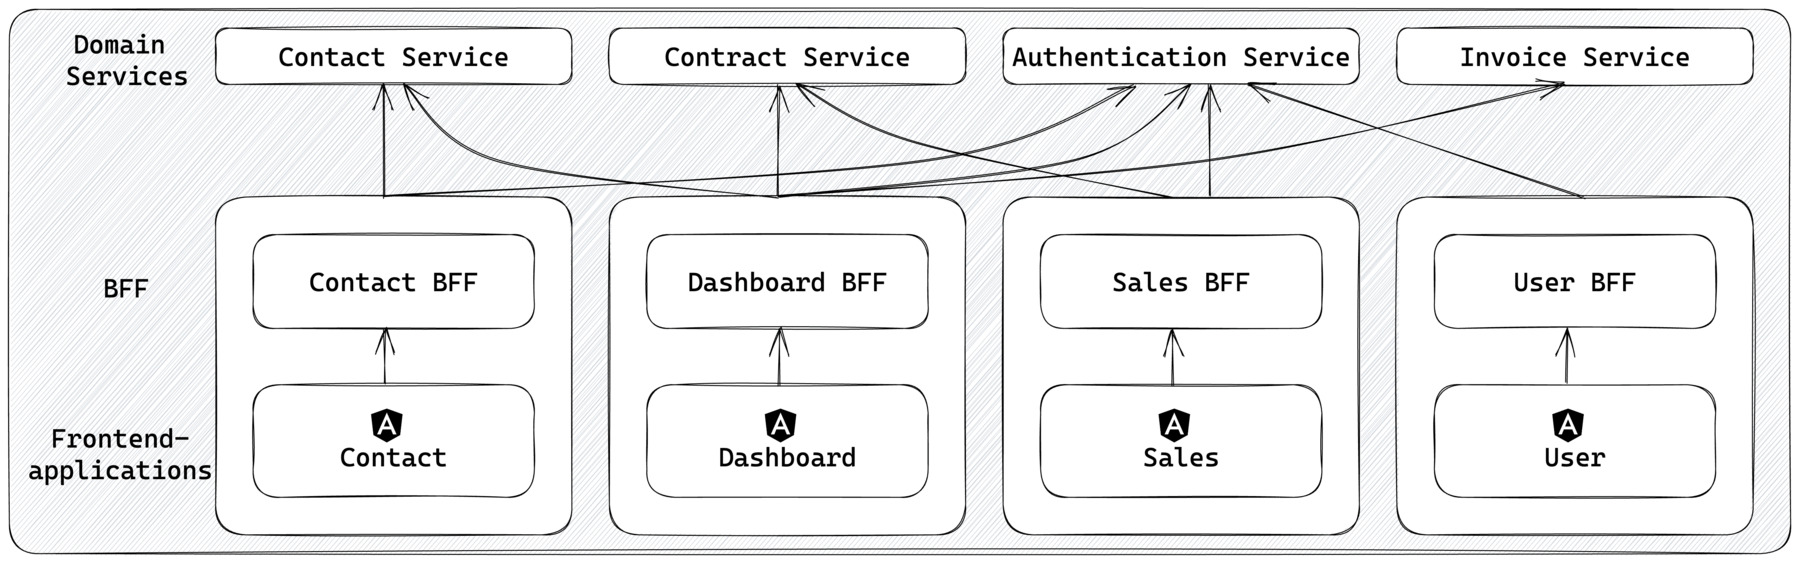
\includegraphics[width=1\linewidth]{images/background/micro-frontends/bff-architecture.jpg}
    \caption{Frontend architecture with the \ac{BFF} pattern.}\label{fig:background:micro-frontend:bff-architecture}
\end{figure}
\fi

\noindent Figure \ref{fig:background:micro-frontend:bff-architecture} shows an exemplary micro-frontend architecture using the \ac{BFF} pattern. Each frontend has a service that retrieves data only for that specific client. Because the \acp{BFF} function as a gateway to the domain services, the domain services can stay very generic and be reused by different clients. \acp{BFF} should implement only the presentation logic that puts the data into the form that the client needs, and it should avoid storing state. \cite{misc:2019:leitner:background:micro-frontends:backend-for-frontends}

\bigskip

\noindent With this architectural approach, the \ac{BFF} and the frontend form a single deployment unit. If one application changes, the other must adapt to the changes. GraphQL is a perfect technology for implementing a \ac{BFF} because it is specifically designed for implementing the presentation layer.

